% !TeX spellcheck = cs_CZ
%{\tikzset{external/prefix={tikz/FYZI/}}
% \tikzset{external/figure name/.add={ch23_}{}}
%=========================== Kapitola: Rezonance ==================================================
\setchaptertoc
\chapter{Rezonance}\label{fyz:IchapXXIII}

  \section{Komplexní čísla a harmonický pohyb}\label{fyz:IchapXXIIIsecI}
  \section{Tlumené nucené kmity}\label{fyz:IchapXXIIIsecII}
  \section{Rezonance v elektrických obvodech}\label{fyz:IchapXXIIIsecIII}
  \section{Rezonance v přírodě}\label{fyz:IchapXXIIIsecIV}
  \section{Příklady a cvičení}\label{fyz:IchapXXIIIsecV}

  \begin{figure}[ht!] %\ref{fyz:fig0415}
    \centering
    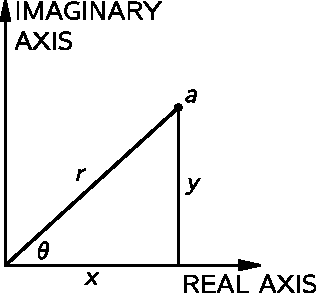
\includegraphics[width=0.3\linewidth]{fyz_fig0415.pdf}
    \caption{Komplexní číslo lze znázornit bodem v \uv{komplexní rovině}
             (\cite[s.~309]{Feynman01})}
    \label{fyz:fig0415}
  \end{figure}

  \begin{figure}[ht!] %\ref{fyz:fig0416}
    \centering
    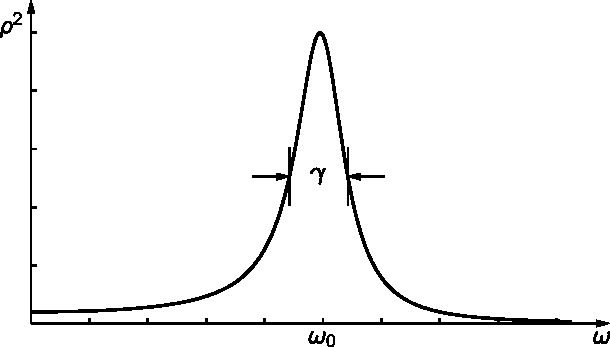
\includegraphics[width=0.7\linewidth]{fyz_fig0416.pdf}
    \caption{Graf \(\varrho^2\) v závislosti na \(\omega\)
             (\cite[s.~313]{Feynman01})}
    \label{fyz:fig0416}
  \end{figure}

  \begin{figure}[ht!] %\ref{fyz:fig0417}
    \centering
    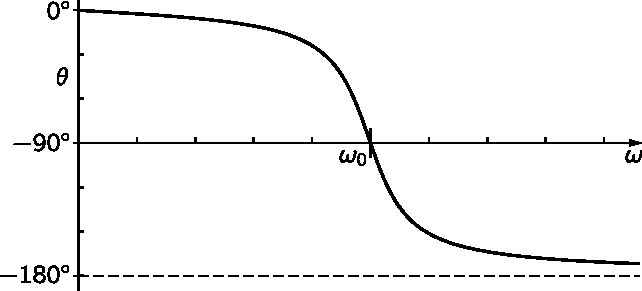
\includegraphics[width=0.7\linewidth]{fyz_fig0417.pdf}
    \caption{Graf \(\vartheta\) v závislosti na \(\omega\)
             (\cite[s.~314]{Feynman01})}
    \label{fyz:fig0417}
  \end{figure}

  \begin{figure}[ht!] %\ref{fyz:fig0418}
    \centering
    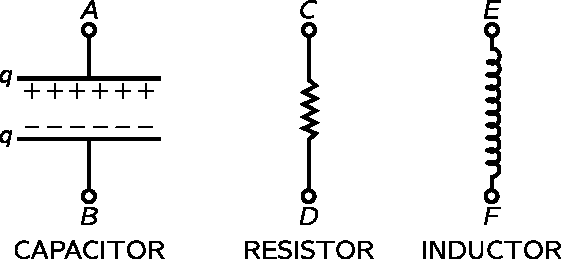
\includegraphics[width=0.5\linewidth]{fyz_fig0418.pdf}
    \caption{Tři pasivní prvky elektrických obvodů
             (\cite[s.~315]{Feynman01})}
    \label{fyz:fig0418}
  \end{figure}

  \begin{figure}[ht!] %\ref{fyz:fig0419}
    \centering
    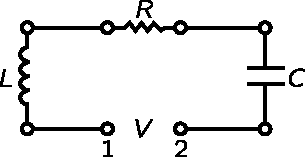
\includegraphics[width=0.3\linewidth]{fyz_fig0419.pdf}
    \caption{Elektrický oscilační obvod s odporem, cívkou a kondenzátorem
             (\cite[s.~316]{Feynman01})}
    \label{fyz:fig0419}
  \end{figure}

  \begin{figure}[ht!] %\ref{fyz:fig0420}
    \centering
    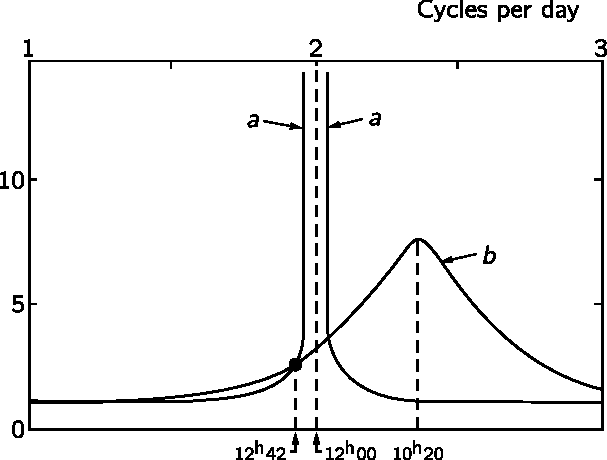
\includegraphics[width=0.7\linewidth]{fyz_fig0420.pdf}
    \caption{Reakce atmosféry na vnější excitace. Křivka \(a\) zobrazuje očekávanou reakci na 
             atmosférický příliv a odliv typu \(S_2\) způsobený gravitací Měsíce: zvětšení v maximu 
             je \(100:1\). Křivka \(b\) představuje průběh odvozený z pozorovaného zvětšení a fáze 
             přílivu a odlivu typu \(M_2\). 
             (\cite[s.~318]{Feynman01})}
    \label{fyz:fig0420}
  \end{figure}

  \begin{figure}[ht!] %\ref{fyz:fig0421}
    \centering
    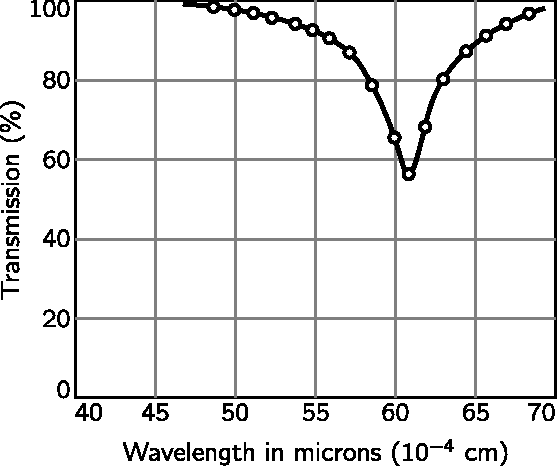
\includegraphics[width=0.7\linewidth]{fyz_fig0421.pdf}
    \caption{Koeficient průchodu infračerveného záření tenkou (\SI{0.17}{\micro\m}) vrstvou 
             chloridu sodného
             (\cite[s.~319]{Feynman01})}
    \label{fyz:fig0421}
  \end{figure}

  \begin{figure}[ht!] %\ref{fyz:fig0422}
    \centering
    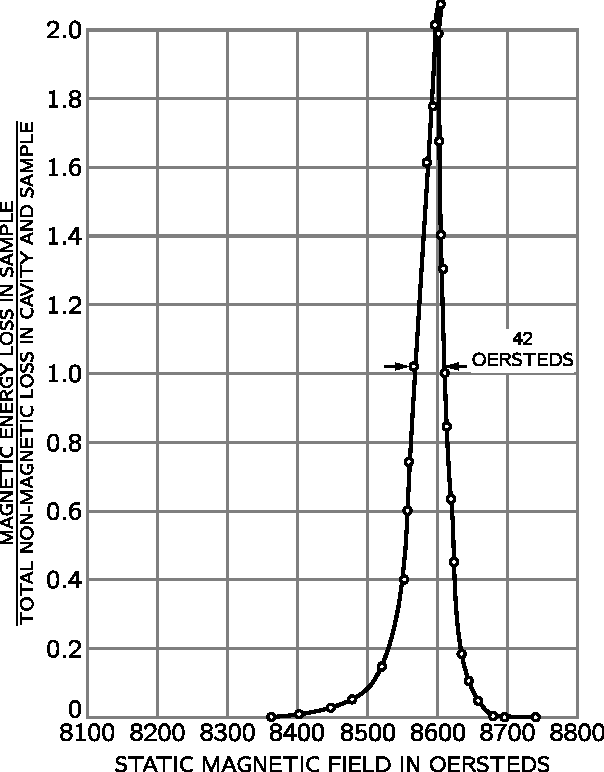
\includegraphics[width=0.7\linewidth]{fyz_fig0422.pdf}
    \caption{Ztráta energie v paramagnetické organické sloučenině v závislosti na intenzitě 
    vnějšího magnetického pole (1 oersted = \SI{1/4\pi e3}{\ampere\per\meter})
             (\cite[s.~320]{Feynman01})}
    \label{fyz:fig0422}
  \end{figure}

  \begin{figure}[ht!] %\ref{fyz:fig0423}
    \centering
    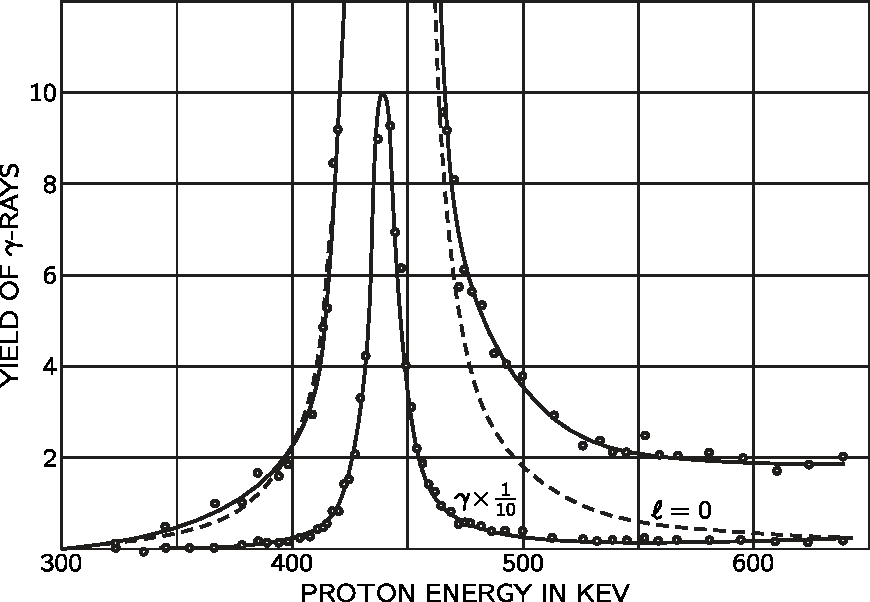
\includegraphics[width=0.7\linewidth]{fyz_fig0423.pdf}
    \caption{Intenzita gama záření lithia jako funkce energie bombardující protonů. Přerušovaná 
             čára představuje teoretický výpočet pro protony s momentem hybnosti \(l=0\)
             (\cite[s.~320]{Feynman01})}
    \label{fyz:fig0423}
  \end{figure}

  \begin{figure}[ht!] %\ref{fyz:fig0424}
    \centering
    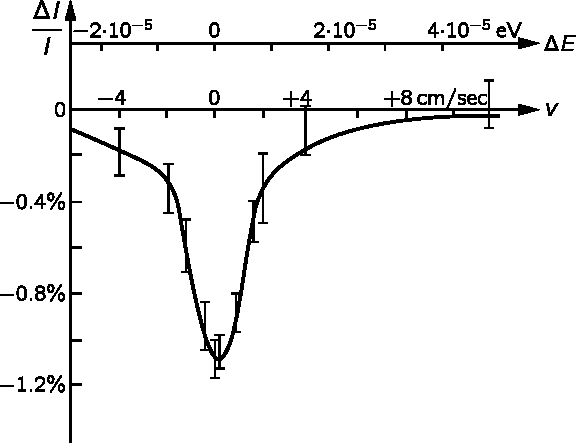
\includegraphics[width=0.7\linewidth]{fyz_fig0424.pdf}
    \caption{S laskavostí Dr. R. M\"{o}ssbauera
             (\cite[s.~321]{Feynman01})}
    \label{fyz:fig0424}
  \end{figure}

  \begin{figure}[ht!] %\ref{fyz:fig0425}
    \centering
    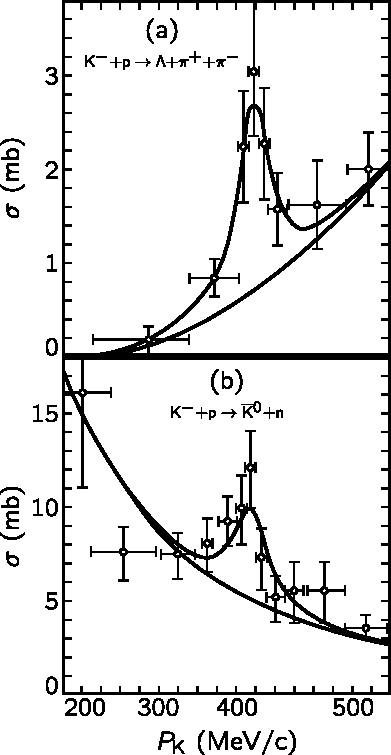
\includegraphics[width=0.6\linewidth]{fyz_fig0425.pdf}
    \caption{Závislost účinného průřezu na hybnosti reakce: a) \(K^+ + p \rightarrow \Lambda + \pi 
    + \pi^-\) b) \(K^- + p \rightarrow K^o + n\); Dolní křivky \(a\) i 
    \(b\) představují předpokládané pozadí bez rezonance, zatímco horní křivky obsahují ještě navíc 
    superponovanou rezonanci; srážkový průřez je v 1 mb = \SI{e-25}{\m\squared}
             (\cite[s.~321]{Feynman01})}
    \label{fyz:fig0425}
  \end{figure}

  \todo[inline]{Kapitola fey1ch23 je zcela prázdná, pouze obrázky}  
%} %tikzset
%---------------------------------------------------------------------------------------------------